\item \textbf{{[}YIJC/PRELIM/9569/2020/P2/Q3{]} }

The task is to store words in nodes that is contained within a linked
list data structure. A node contains a word, the word category and
a next pointer. The pointers link the word items in proper grammatical
order based on their word category (\textquoteleft N\textquoteright :
noun, \textquoteleft V\textquoteright : verb, \textquoteleft D\textquoteright :
determiner, \textquoteleft J\textquoteright : adjective). The unused
nodes are linked as shown below. The first unused node is the position
where the new word item is to be stored.
\begin{center}
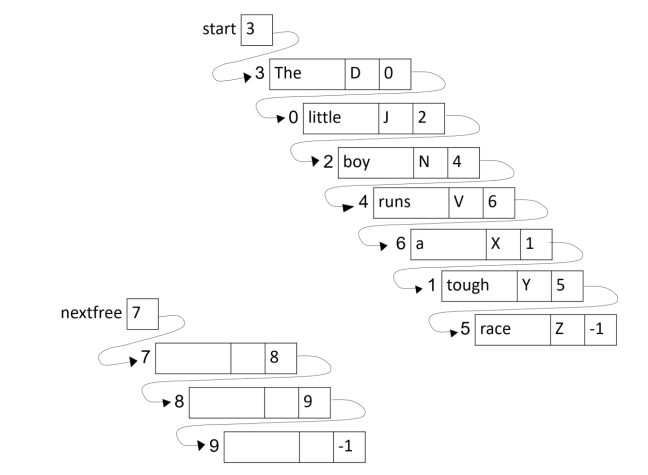
\includegraphics[width=0.5\paperwidth]{C:/Users/Admin/Desktop/Github/question_bank/LyX/static/img/9569-YIJC-2020-P2-Q3-1}
\par\end{center}

The diagram shows the linked list with:
\begin{itemize}
\item the words and their respective category inserted in the following
order: 
\begin{itemize}
\item \texttt{'little', 'J' }
\item \texttt{'tough', 'J' }
\item \texttt{'boy', 'N' }
\item \texttt{'The', 'D' }
\item \texttt{'runs', 'V' }
\item \texttt{'race', 'N' }
\item \texttt{'a', 'D'}
\end{itemize}
\item the unused nodes linked together
\end{itemize}
Each node is implemented as an instance of the class Node. The class
Node has the following UML class diagram:
\begin{center}
\begin{tabular}{|l|}
\hline 
\hspace{0.25\columnwidth}Node\tabularnewline
\hline 
\texttt{word: STRING}\tabularnewline
\texttt{category: STRING}\tabularnewline
\texttt{next: INTEGER}\tabularnewline
\hline 
\texttt{constructor()}\tabularnewline
\texttt{set\_word(w: STRING)}\tabularnewline
\texttt{set\_category(c: STRING)}\tabularnewline
\texttt{set\_next(n: INTEGER)}\tabularnewline
\texttt{get\_word(): STRING}\tabularnewline
\texttt{get\_category(): STRING}\tabularnewline
\texttt{get\_next(): INTEGER}\tabularnewline
\hline 
\end{tabular}
\par\end{center}

The \texttt{LinkedList} class is implemented as follows: 
\begin{itemize}
\item Attributes
\begin{itemize}
\item \texttt{sentence : ARRAY{[}0:9{]} of Node -} The linked list data
structure that contains 10 nodes.
\item \texttt{start : INTEGER} - Index for the start position of the linked
list. 
\item \texttt{nextfree : INTEGER} - Index for the next unused node.
\end{itemize}
\item Methods
\begin{itemize}
\item \texttt{\_\_init\_\_ : PROCEDURE} - Sets all the node data values
to \textquoteleft empty string\textquoteright . Set pointers to indicate
all nodes are unused and linked. Initialise values for start and nextfree.
\item \texttt{isempty : FUNCTION RETURNS BOOLEAN} - Tests for empty linked
list.
\item \texttt{isfull : FUNCTION RETURNS BOOLEAN} - Tests for no unused nodes.
\item \texttt{display : PROCEDURE} - Displays the contents of sentence in
index order. 
\item \texttt{insert : PROCEDURE} - Adds a new word and its category to
the linked list. 
\item \texttt{traversal : PROCEDURE} - Displays the simple sentence obtained
from the linked list.
\end{itemize}
\end{itemize}
The index of the first available node is indicated by \texttt{nextfree}.
The initial values of \texttt{start} and \texttt{nextfree} is -1 and
0 respectively.

\subsection*{Task 3.1}

Write the program code to define the \texttt{Node} and \texttt{LinkedList}
classes. 

Do not attempt to write the methods \texttt{insert} and \texttt{traversal}
at this stage. \hfill{} {[}10{]}

\subsection*{Task 3.2}

Write program code to create a LinkedList object and run the display
method to confirm the initial values of the pointers, word and category
values when the linked list is empty. \hfill{}{[}2{]}

A simple sentence contains words from different category arranged
in the manner as illustrated: 

(\textquoteleft N\textquoteright : noun, \textquoteleft V\textquoteright :
verb, \textquoteleft D\textquoteright : determiner, \textquoteleft J\textquoteright :
adjective)

Verb come between two nouns.

Determiner comes before a noun, adjective comes before a noun and
after a determiner.
\noindent \begin{center}
\begin{tabular}{|c|c|c|}
\hline 
boy & runs & race\tabularnewline
\hline 
N & V & N\tabularnewline
\hline 
\end{tabular}
\par\end{center}

\noindent \begin{center}
\begin{tabular}{|c|c|c|c|c|}
\hline 
The & boy  & runs & a & race\tabularnewline
\hline 
D & N & V & D & N\tabularnewline
\hline 
\end{tabular}
\par\end{center}

\noindent \begin{center}
\begin{tabular}{|c|c|c|c|c|c|c|}
\hline 
The & little & boy & runs & a & tough & race\tabularnewline
\hline 
D & J & N & V & D & J & N\tabularnewline
\hline 
\end{tabular}
\par\end{center}

In order to aid the process of inserting the words in their correct
position in the linked list, the code letter \textquoteleft X\textquoteright ,
\textquoteleft Y\textquoteright{} and \textquoteleft Z\textquoteright{}
is used in place of the second set of \textquoteleft D\textquoteright ,
\textquoteleft J\textquoteright , \textquoteleft N\textquoteright{}
respectively, so that the correct position can be determined by comparing
the category when traversing down the linked list.
\noindent \begin{center}
\begin{tabular}{|c|c|c|c|c|c|c|}
\hline 
The & little & boy & runs & a & tough & race\tabularnewline
\hline 
D & J & N & V & X & Y & Z\tabularnewline
\hline 
\end{tabular}
\par\end{center}

The following pseudocode (available in PSEUDOCODE\_TASK\_3\_3.TXT
) can be used to add a word and its category to the linked list.

\noindent %
\noindent\begin{minipage}[t]{1\columnwidth}%
\texttt{PROCEDURE insert(new\_word, new\_category)}

\texttt{\bigskip{}
}

\texttt{\qquad{}//check if Linked List is full }

\texttt{\qquad{}IF nextfree = -1 THEN }

\texttt{\qquad{}\qquad{}RETURN 'Linked List is Full' }

\texttt{\qquad{}ENDIF }

\texttt{\bigskip{}
}

\texttt{\qquad{}//linked list is not full, safe to insert new word }

\texttt{\qquad{}sentence{[}nextfree{]}.word <- new\_word }

\texttt{\qquad{}sentence{[}nextfree{]}.category <- new\_category}

\texttt{\bigskip{}
}

\texttt{\qquad{}IF start = -1 THEN //inserting into empty list }

\texttt{\qquad{}\qquad{}start <- nextfree}

\texttt{\qquad{}\qquad{}temp <- sentence{[}start{]}.next }

\texttt{\qquad{}\qquad{}sentence{[}start{]}.next <- -1 }

\texttt{\qquad{}\qquad{}nextfree <- temp}

\texttt{\bigskip{}
}

\texttt{\qquad{}ELSE }

\texttt{\qquad{}// traverse down the linked list to search for position
to}

\texttt{\qquad{}// insert }

\texttt{\qquad{}\qquad{}current <- start //pointer of current node }

\texttt{\qquad{}\qquad{}previous <- -1 //pointer of previous node }

\texttt{\qquad{}\qquad{}inserted <- FALSE //flag to check for insertion}

\texttt{\bigskip{}
}

\texttt{\qquad{}\qquad{}WHILE current > -1 AND inserted = FALSE}

\texttt{\qquad{}\qquad{}\qquad{}IF sentence{[}current{]}.category
> new\_category THEN \bigskip{}
}

\texttt{\qquad{}\qquad{}\qquad{}//position found, insert before
current node }

\texttt{\qquad{}\qquad{}\qquad{}\qquad{}IF current = start THEN }

\texttt{\qquad{}\qquad{}\qquad{}\qquad{}\qquad{}//check if current
equals to start}

\texttt{\qquad{}\qquad{}\qquad{}\qquad{}\qquad{}start <- nextfree }

\texttt{\qquad{}\qquad{}\qquad{}\qquad{}ELSE }

\texttt{\qquad{}\qquad{}\qquad{}\qquad{}\qquad{}sentence{[}previous{]}.next
<- nextfree}

\texttt{\qquad{}\qquad{}\qquad{}\qquad{}ENDIF \bigskip{}
}

\texttt{\qquad{}\qquad{}\qquad{}\qquad{}temp <- sentence{[}nextfree{]}.next}

\texttt{\qquad{}\qquad{}\qquad{}\qquad{}sentence{[}nextfree{]}.next
<- current}

\texttt{\qquad{}\qquad{}\qquad{}\qquad{}nextfree <- temp}

\texttt{\qquad{}\qquad{}\qquad{}\qquad{}inserted <- TRUE}

\texttt{\bigskip{}
}

\texttt{\qquad{}\qquad{}\qquad{}ELIF sentence{[}current{]}.category
< new\_category THEN }

\texttt{\qquad{}\qquad{}\qquad{}\qquad{}previous <- current }

\texttt{\qquad{}\qquad{}\qquad{}\qquad{}current <- sentence{[}current{]}.next }

\texttt{\bigskip{}
}

\texttt{\qquad{}\qquad{}\qquad{}ELSE THEN }

\texttt{\qquad{}\qquad{}\qquad{}\qquad{}IF new\_category = 'N'
THEN }

\texttt{\qquad{}\qquad{}\qquad{}\qquad{}\qquad{}new\_category
<- 'Z'}

\texttt{\qquad{}\qquad{}\qquad{}\qquad{}ENDIF }

\texttt{\qquad{}\qquad{}\qquad{}\qquad{}IF new\_category = 'D'
THEN }

\texttt{\qquad{}\qquad{}\qquad{}\qquad{}\qquad{}new\_category
<- 'X' }

\texttt{\qquad{}\qquad{}\qquad{}\qquad{}ENDIF }

\texttt{\qquad{}\qquad{}\qquad{}\qquad{}IF new\_category = 'J'
THEN }

\texttt{\qquad{}\qquad{}\qquad{}\qquad{}\qquad{}new\_category
<- 'Y' }

\texttt{\qquad{}\qquad{}\qquad{}\qquad{}ENDIF }

\texttt{\bigskip{}
}

\texttt{\qquad{}\qquad{}\qquad{}\qquad{}previous <- current }

\texttt{\qquad{}\qquad{}\qquad{}\qquad{}current <- sentence{[}current{]}.next}

\texttt{\qquad{}\qquad{}\qquad{}\qquad{}sentence{[}nextfree{]}.category
<- new\_category}

\texttt{\qquad{}\qquad{}\qquad{}ENDIF}

\texttt{\qquad{}\qquad{}ENDWHILE}

\texttt{\bigskip{}
}

\texttt{\qquad{}\qquad{}IF inserted = False THEN }

\texttt{\qquad{}\qquad{}\qquad{}sentence{[}previous{]}.next <-
nextfree }

\texttt{\qquad{}\qquad{}\qquad{}temp <- sentence{[}nextfree{]}.next }

\texttt{\qquad{}\qquad{}\qquad{}sentence{[}nextfree{]}.next <-
-1 }

\texttt{\qquad{}\qquad{}\qquad{}nextfree <- temp }

\texttt{\qquad{}\qquad{}ENDIF }

\texttt{\bigskip{}
}

\texttt{\qquad{}ENDIF}

\texttt{ENDPROCEDURE}%
\end{minipage}

\subsection*{Task 3.3}

Write code to implement \texttt{insert} method from this pseudocode.
You may use the text file \texttt{PSEUDOCODE\_TASK\_3\_3.TXT} as a
basis for writing your code. \hfill{}{[}8{]}

\subsection*{Task 3.4:}

Write code to insert the following into the linked list created in
\textbf{Task 3.2} and display its contents:
\begin{itemize}
\item 'little', 'J' 
\item 'tough', 'J' 
\item 'boy', 'N' 
\item 'The', 'D' 
\item 'runs', 'V' 
\item 'race', 'N' 
\item 'a', 'D' \hfill{}{[}2{]}
\end{itemize}

\subsection*{Task 3.5:}

Write code to implement traversal method which displays the simple
sentence obtained from traversing the linked list and run it. 

The expected output should look like this:
\noindent \begin{center}
\texttt{The little boy runs a tough race. }\hfill{}{[}8{]}
\par\end{center}

Download your program code and output for Task 3 as

\texttt{Task3\_<your name>\_<centre number>\_<index number>.ipynb}